%% content.tex
%%


%% ===========================
\chapter{Umsetzung}
%% ===========================

%% ===========================
\section{Erzeugung der Abfrage}
%% ===========================

Um Abfragen durch den Benutzer möglichst performant zu beantworten erfolgt die Erzeugung dynamisch. Das bedeutet die SQL-Abfrage an die Datenbank kann je nach Anforderung anders aufgebaut sein. Die Kernaufgabe ändert sich jedoch nie. Diese besteht aus der Bildung von Summen basierend auf verschiedenen Verbindungstypen. Zu Berücksichtigen ist das jede Abfrage einen Anfangs- und Endzeitpunkt enthält und somit beachtet werden muss. Nachdem festgestellt wurde wie viele Verbindungen von den jeweiligen Typen zu einer Person verlaufen wird zusätzlich die Gesamtsumme der Verbindungen zu einer Person gebildet. Die Summe wird zur Sortierung der Ergebnisse verwendet. Bei der Sortierung wird absteigend vorgegangen um die Personen mit den meisten Verbindungen zu der von der Suche ausgehend Person zu ermitteln. Das Ergebnis wird wiederum auf eine durch den Benutzer festgelegte Anzahl reduziert. 

Zu diesen Kernfunktionalitäten können durch Angaben des Nutzers weitere hinzukommen. Eine von Ihnen ist die Gewichtung von Zeitpunkten. Der Ansatz zur Umsetzung der Gewichtung der Zeit wird anhand der Abbildung \ref{fig:umsetzung:gewichtungderzeit} erklärt. Die Abbildung zeigt ein Koordinatensystem mit den Gewichtung von einzelnen Zeitpunkten. Die x-Achse stellt den zeitlichen Verlauf dar. Während die y-Achse die Gewichtung darstellt. $t_{start}$ markiert den Startzeitpunkt, wohingegen $t_{end}$ den Endzeitpunkt angibt. Mithilfe von $t_1$ und $t_2$ werden Zeitspannen festgelegt, die differenziert zu gewichten sind. Um nun die Tage zu gewichten wurde der lineare Ansatz gewählt. Das bedeutet zwischen $t_{start}$ und $t_1$ steigt die Relevanz stetig bis sie die 100 Prozent erreicht hat. Ab dort sind alle Tage wieder 100 Prozent relevant außer es ist ein $t_2$ angegeben worden. Falls ja wird ab $t_2$ linear fallend, jeder Tag bewertet. 

Zur Berechnung der Gewichtung zu einem bestimmten Tag werden die folgenden zwei Variablen verwenden:

\begin{equation}
f_1 = \frac{1}{t_1 - t_{start}}
\end{equation}
\begin{equation}
f_2 = \frac{1}{t_{end} - t_2}
\end{equation}

Dabei wird wie folgt vorgegangen. $t_{start}$ markiert Tag. Aufsteigend zählend wird jeder Tag bis $t_1$ mit der Variabel $f_1$ multipliziert. Für den Zeitpunkt $t_2$ wird die Summe der Tage in der Zeitspanne zwischen $t_2$ und $t_{end}$ verwendet. Die Summe wird mit jedem weiteren Tag um 1 vermindert bis zum Zeitpunkt $t_{end}$, der 0 darstellt. Bei jedem Schritt wird der Tag mit der Variablen $f_2$ multipliziert.

\begin{figure}[htbp]
\begin{center}
\begin{tikzpicture}[domain=-1:2] \draw[very thin,color=gray] (0,0); 
\draw[->] (0,0) -- (12.3,0) node[right] {Zeit}; 
\draw[->] (0,0) -- (0,4.2) node[above] {Faktor Gewichtung}; 
\draw[color=black]  (0.2,3) -- (-0.2,3)   node[left] {100\%};
\draw[color=black]  (0.2,1.5) -- (-0.2,1.5)   node[left] {50\%};  
\draw[dashed][color=black]  (5,0.5) -- (5,3.5); 
\draw[dashed][color=black]  (9,0.5) -- (9,3.5);

\draw[color=black]  (0,0) -- (0,0)   node[below] {$t_{start}$}; 
\draw[color=black]  (5,0.1) -- (5,-0.1)   node[below] {$t_1$}; 
\draw[color=black]  (9,0.1) -- (9,-0.1)   node[below] {$t_2$};
\draw[color=black]  (12,0.1) -- (12,-0.1)   node[below] {$t_{end}$};   
 
\draw[color=black]  (0,0) -- (5,3)   node[right] {}; 
\draw[color=black]  (5,3) -- (9,3)   node[right] {}; 
\draw[color=black]  (9,3) -- (12,0)   node[right] {};  

\end{tikzpicture} 
\end{center}
\caption{Gewichtung der Zeit}
\label{fig:umsetzung:gewichtungderzeit}
\end{figure}

Neben der Gewichtung der Zeit lassen sich die jeweiligen Verbindungstypen unterschiedlich gewichten. Bei einer Abweichung von 100 Prozent wird die Summe des jeweiligen Verbindungstypen um die durch den Nutzer bestimmten Prozentsatz verringert. 

Die restlichen Parameter dienen der Filterungen und werden je nach Nutzer-Eingabe zu den Bedingungen der SQL-Abfrage hinzugenommen. Unter Ihnen gibt es eine Bedingung zuvor Ermittelt werden muss und daher näher beschrieben wird. Dabei handelt es sich um das ausschließen von Gruppen, da sich Ihre Zusammensetzung über die Zeit variabel ist. Dazu wird die Tabelle UserGroup verwendet. Dabei wird wie folgendermaßen vorgegangen. Zuerst wird die Ergebnismenge auf die ausgewählten Gruppen reduziert. Anschließend wird für jede Gruppe ein eigener Container erzeugt, der alle Personen der Gruppe enthält. Liegt nun das Feld Date nach dem Anfangszeitpunkt der Abfrage und die Spalte Action enthält eine 1, wird der Container um diese Person reduziert. Enthält die Spalte Action eine 0 wird die Person zum Container hinzugefügt. Die 1 in der Spalte Action bedeutet das die Person zu dem in der Spalte Date angegeben Datum die Gruppe verlassen hat. Eine 0 bedeutet das die Person zu dem angegeben Datum hinzukam. Dadurch wird die Zusammensetzung zum Anfangszeitpunkt wiederhergestellt. Mithilfe der Personen aus den Container wird nun die SQL-Abfrage um weitere Bedingungen erweitert.

Zu beachten ist natürlich das innerhalb des Zeitraums Gruppenveränderungen stattgefunden haben können, diese jedoch nicht zu Berücksichtigen sind. Es kann jeweils nur ein bestimmter Zeitpunkt für die Betrachtung berücksichtigt werden. In diesem Fall wurde der Anfangszeitpunkt gewählt.

%% ===========================
\section{ETL Prozess}
%% ===========================

Um an die notwendigen Daten zu gelangen werden zuerst die Informationen aus der alten Datenbank extrahiert. Dazu wird ein Verbund gebildet der die Tupeln der Tabellen verschmelzen lässt. Die manuellen erstellten Verbindungen in der alten Datenbank werden mithilfe der Tabelle TableRelation festgehalten. Zur Gewinnung dieser Verbindungen wird als erstes eine SQL-Abfrage definiert die für jede der Tabellen gwOpportunity, gwPhoneCall0, Document0, EmailStore0 und Appointment0 separat ausgeführt wird. 

Mithilfe des ersten Verbundes zwischen SysUser und Adresse wird die Adresse einer Person ermittelt. Anschließend wird durch einen Verbund der TableRelation und SysUser alle Tabellen ermittelt die mit der Person eine Verbindung besitzen. Der nächste Verbund ist zwischen TableRealtion und einer der fünf zuvor genannten Tabellen. Um festzustellen welche Personen auch mit beispielsweise einem Dokument arbeiten zu ermitteln wird ein weiterer Verbund mit der passenden ORel-Tabelle ausgeführt. In der ORel-Tabelle kann die OID positiv sowie negativ sein. Bei einem negativen Wert stellt die OID eine GID der Tabelle SysGroup dar. Zur Auflösung der Gruppe in einzelne Personen werden folgende Verbunde gebildet. Zuerst zwischen SysGroup und SysGroupMember um alle Personen die zu einer Gruppe gehören zu erhalten. Anschließend zwischen SysGroupMember und SysUser um die OID der Person zu erhalten. 

Nachdem alle Information in einem Verbund vorhanden sind werden lediglich drei Informationen des Gesamten Verbundes behalten. Zu einem die OID des SysUser von dem die Suche ausgeht. Zum anderen das Datum welches durch das Objekt welches die Personen verbindet ermittelt wird. Weiterhin wird die zweite OID durch den Verbund mit einer zweiten SysUser Tabelle behalten. Zum Schluss wird manuell eine vierte Information beigefügt die besagt welchem Objekt die Tupel entstammt. 

Für den Sonderfall das ein Datum über mehrere Tage geht wird eine fünfte Spalte hinzugefügt welche den Zeitraum in Tagen beinhaltet. Zur Beschaffung der geschobenen Termine wird genau wie in der Konzeption beschrieben verfahren.

Zur Ermittlung direkter Verbindungen zwischen Personen wird lediglich ein Verbund aus zwei ORel-Tabellen eines Objektes gebildet. Dieser Verbund beinhaltet bereits die OIDs der beiden Personen. Zur Ermittlung des Datums wird noch ein Verbund mit der Tabelle des Objektes gebildet. Die negativen OIDs werden genauso wie oben beschrieben aufgelöst. 

Jede Antwort einer SQL-Abfrage zur Gewinnung von Daten wird in einer SCV-Datei direkt auf dem Tomcat Server abgelegt. Diese CSV Dateien stellen die Grundlage der Transformation dar. Jede dieser Dateien beinhaltet Verbindungen zwischen Personen in der Form wie sie Abbildung \ref{fig:umsetzung_csv_datei} zeigt. 

\begin{figure}[htbp]
\begin{center}
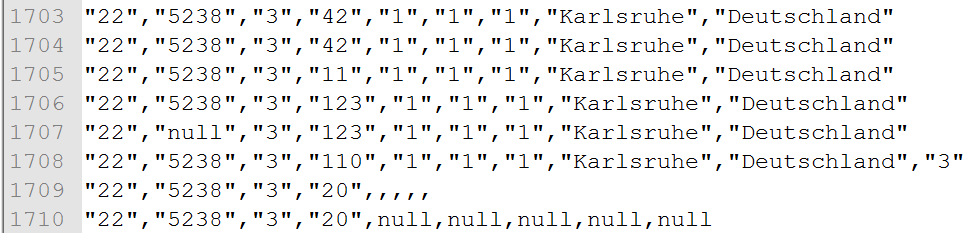
\includegraphics[width=1.0\textwidth]{pics/umsetzung_csv_datei.png}
\caption{Ausschnitt einer CSV-Datei mit Daten der Extraktion}
\label{fig:umsetzung_csv_datei}
\end{center}
\end{figure}

Alle CSV-Dateien werden auf die in Abbildung \ref{fig:umsetzung_csv_datei} zu sehenden Ungereimtheiten untersucht. Dabei werden Zeilen wo die letzten fünf Werte fehlen über die die OID (die vierte Zahl) die Adresse ergänzt. Bei null Werten wird überprüft ob wirklich keine Adresse vorhanden ist falls doch werden diese ebenfalls ergänzt. Wenn wie in Zeile 1707 zu sehen eine null Anstatt einem Datum steht wird die Zeile entfernt. Falls wie in Zeile 1708 ein zusätzlicher zehnter Wert vorhanden ist, bedeutet das die Verbindung über mehrere Tage geht. Die Zeile bleibt bestehen jedoch wird der letzte Wert entfernt. Die Zahl wird jedoch noch verwendet um die weiteren Zeilen mit aufsteigendem Datum zu erzeugen. Nach der Beseitigung von Anomalien werden noch die Städte und Länder durch ihre jeweilige ID aus der Tabelle Town und Country ersetzt.

Die veränderten Daten werden wieder in CSV-Dateien abgelegt die gleich bezeichnet sind allerdings noch den Zusatz "\_transf" besitzen der Sie als Transformiert  markiert. Diese Dateien werden anschließend in eine CSV-Datei zusammengeführt. Bei der Zusammenführung sind zum ersten mal alle Daten gleichzeitig in der Anwendung weshalb an dieser Stelle alle Duplikate beseitigt werden. Weiterhin werden die Zeilen sortiert. Dabei wird mit zwei Kriterien sortiert. Das erste Kriterium ist der Erste Wert die OID der Person von dem die Suche ausgeht. Wenn hierbei gleiche Werte verglichen werden wird das zweite Feld(Datum) herangezogen. Nachdem alle Zeilen sortiert und von Duplikaten bereinigt sind werden alle Zeilen in einer CSV-Datei abgelegt. 

Diese Datei wird bei jedem Start des Tomcats dazu verwendet einen Bulk-Load für die H2-Datenbank zu initialisieren. Nachdem die Datenbank mit Daten befüllt wurde werden abschließend die Indizes erzeugt.

%% ===========================
\section{Aufbau der Server.war}
%% ===========================

Das Server Web Archive beinhaltet ein dynamisches Web Projekt aus dem Eclipse Web Tools Platform (WTP) Projekt. Das Project weist die typische Struktur eines Web Projektes auf. Daher wird im folgenden nur auf die Klassen eingegangen. Abbildung \ref{umsetzung_klassendiagramm_server} zeigt das Klassendiagramm der Server.war. Das Diagramm dient als Basis für die nachfolgenden Erläuterungen. 

Die H2-Datenbank wird im Embedded-Modus betrieben, was eine Instanziierung der Datenbank zur Laufzeit notwendig macht. Die Instanziierung erfolgt in der Klasse Database. Das Attribut dataSource stellt die H2-Datenbank in Form eines Objektes dar. Eine Verbindung zur Datenbank wird mithilfe der Methode .getConnection() aufgebaut. Diese Verbindung wird permanent offen gehalten solang der Tomcat Server läuft. Dazu wird die Verbindung dem Attribut con zugewiesen, die von allen Methoden verwendet wird die eine Verbindung zur Datenbank aufbauen wollen. Um die Datenbank mit dem deployen der Web-Anwendungen zu starten, ist die Verwendung eines Servlets nötig. Dazu benutzen wir die Klasse EntryPoint die das Interface HttpServlet implementiert. Um das Servlet direkt beim Start aufzurufen wird in der web.xml folgende Zeilen eingetragen: 

\begin{lstlisting}[language=XML]
	<servlet>
		<servlet-name>H2</servlet-name>
		<servlet-class>de.cas.db.EntryPoint</servlet-class>
		<load-on-startup>1</load-on-startup>
	</servlet>
\end{lstlisting}

Die 1 im Element <load-on-startup> bewirkt den Aufruf der Methode init() die eine Instanziierung der Klasse Database vornimmt. Zur Erzeugung des Schemas wird eine separate Klasse namens SchemaBuilder eingesetzt. In Ihr werden sämtliche SQL-Anweisungen zur Generierung des Schemas aufbewahrt und können über die Methode createSchema() ausgeführt werden.

Mit der Klasse JerseyServer wird der REST-Server umgesetzt. Sie besitzt Methoden die mit dne entsprechenden Annotationen wie @GET oder @OST die REST-Requests entgegen nehmen. Mit der Annotation @Path wird die URL angegeben unter der die Methode angesprochen werden kann. Diese Methoden können Übergabeparameter vom Typ UriInfo und/oder HttpHeaders besitzen, die Abrufe von Metadaten der REST-Requests ermöglichen. 

\begin{figure}[htbp]
\begin{center}
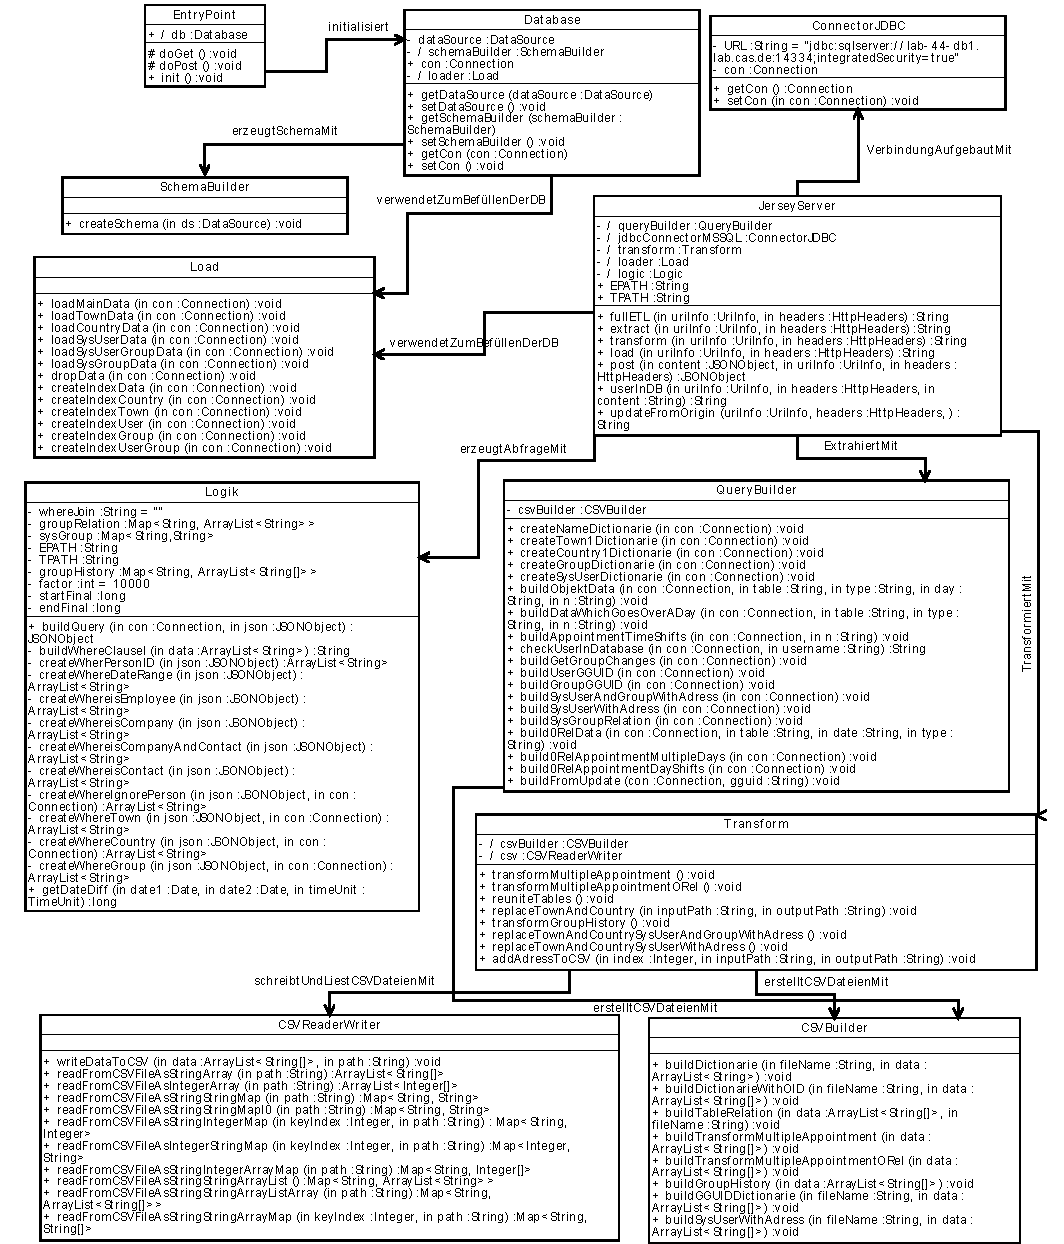
\includegraphics[width=1.0\textwidth]{pics/ServerKlassendiagramm.pdf}
\caption{Server Klassendiagramm}
\label{umsetzung_klassendiagramm_server}
\end{center}
\end{figure}

Neben den Methoden zu Beantwortung von REST-Requests, enthält die Klasse alle Objekte zur Durchführung des ETL-Prozesses. Die Klasse ConnectorJDBC besitzt ein Attribut namens con welches den Verbindungsaufbau zum MSSQL Server mithilfe von JDBC ermöglicht. Zur Extraktion der Daten aus dem MSSQL 2008 wird ein Objekt der Klasse QueryBuilder verwendet. Wie in der Abbildung zu sehen werden für die verschiedenen Tabellen des neuen Schemas, jeweilige Methoden zur Verfügung gestellt. Methoden welche die Übergabewerte table, date und n besitzen, werden für die verschiedenen Verbindungsobjekte benötigt. Mithilfe des Parameters table wird der Name der Tabelle in der MSSQL Datenbank übergeben. Der Parameter date gibt das Feld an was für die Ermittlung des Datums verwendet werden soll. Um den Typ einer Verbindung zwischen Personen festzuhalten wird der Parameter n verwendet, der eine Zahl zwischen eins und fünf beinhaltet. QueryBuilder verwendet ein Objekt vom Typ CSV-Builder um die Ergebnisse in Dateien festzuhalten. Den Methoden wird als Übergabeparameter ein Dateiname sowie die Daten selbst übergeben.


%% ===========================
\section{Aufbau der Client.war}
%% ===========================

\begin{figure}[htbp]
\begin{center}
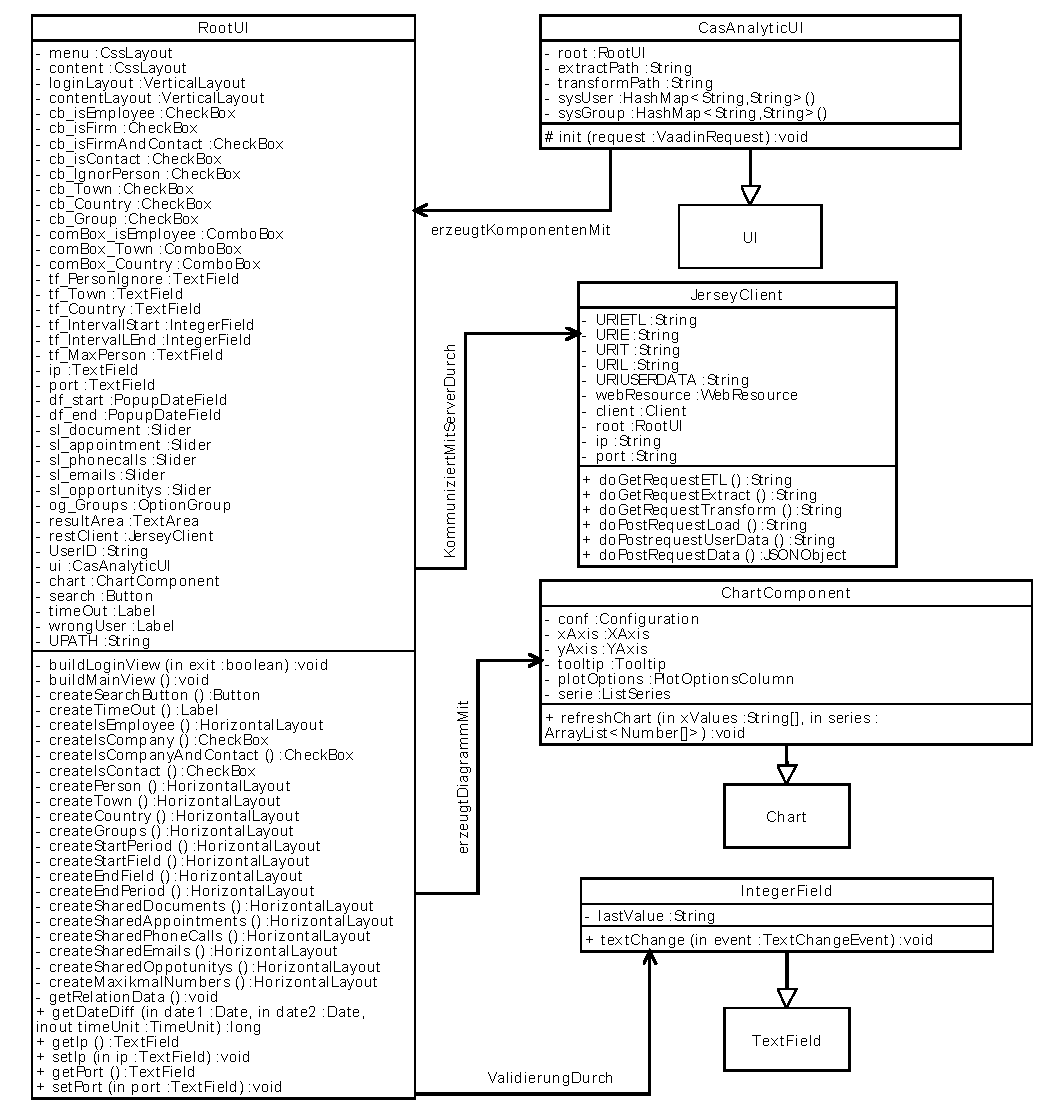
\includegraphics[width=1.0\textwidth]{pics/ClientKlassendiagramm.pdf}
\caption{Client Klassendiagramm}
\label{umsetzung_klassendiagramm_client}
\end{center}
\end{figure}